\section{Adapter}

\begin{figure}[h]
\centering
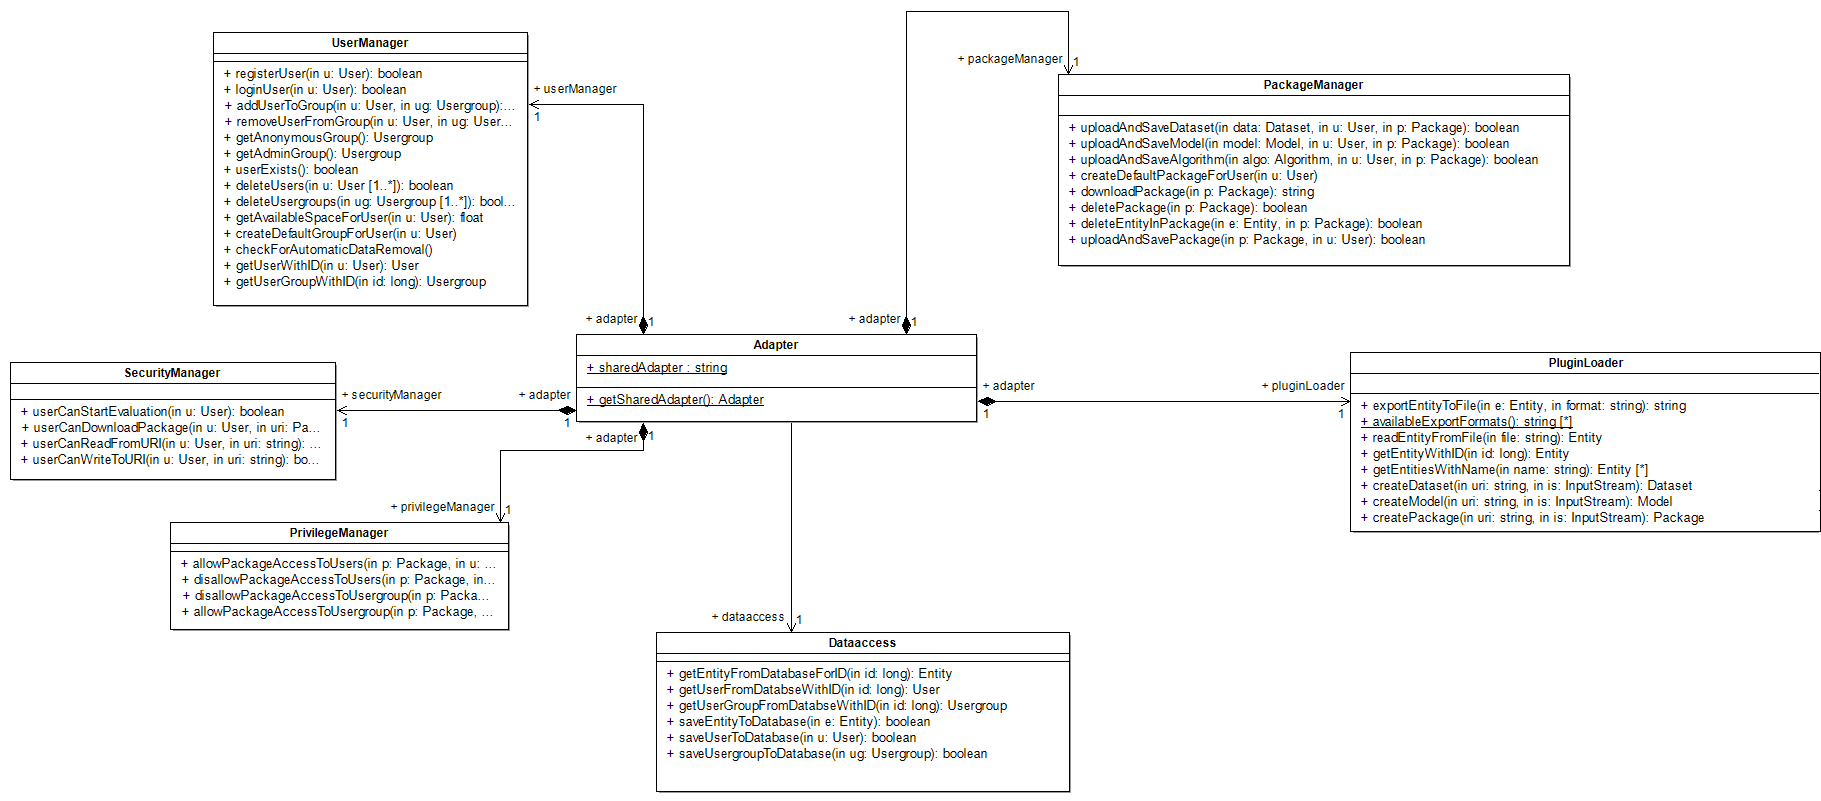
\includegraphics[width=1.0\linewidth]{Grafik/Klassendiagramme/adapter.png}
\end{figure}

Der Adapter implementiert das Singleton-Pattern, d.h. es existiert immer nur genau eine einzige Instanz der Adapterklasse. Hierbei kennt der Adapter je eine einzige Instanz der jeweiligen Kernkomponenten des Systems. Durch diese Implementierung ist ein Zugriff auf sämtliche dieser Komponenten leicht von verschiedenen Klassen aus möglich. Stellt der Nutzer beispielsweise eine Anfrage an das System, so erhalten die Klassen der Präsentationsebene über den Adapter eine Instanz der jeweils notwendigen Managerklasse, wie z.B. dem UserManager.